\documentclass[a4paper]{article}
\usepackage{graphicx}
\begin{document}
\section{JSON}
\subsection{Definisi JSON}
JSON atau JavaScript Object Notation adalah salah satu bentuk format yang ringkas untuk melakukan pertukaran sebuah data di dalam computer. JSON sendiri berbasis teks dan mudah untuk dibaca oleh manusia serta dapat digunakan untuk representasi struktur data sederhana JSON juga dapat digunakan untuk proses transmisi data terstruktur melalui media koneksi jaringan yang disebut Serialisasi.
\subsection{Definisi JSON}
JSON  adalah  bagian  dari  sebuah bahasa  pemrograman  JavaScript  JSON juga merupakan format teks yang sepenuhnya independen tetapi menggunakan konvensi yang  familiar  dengan  bahasa  pemrograman  dari  parent-C,  termasuk  bahasa C,  Java,  Java Script,  Perl, Python,  dan lain sebagainya.  Kelebihan  inilah  yang  membuat  JSON  menjadi  sebuah  bahasa yang disebut  data-interchange yang ideal.
\subsection{Struktur pada JSON}
JSON memiliki 2 struktur,yaitu:
1.	Kumpulan pasangan nama/nilai.
Dalam beberapa Bahasa pemrograman, ini biasanya sering disebut seperti objek, rekaman, struktur, kamus, tabel hash, daftar berkunci atau array assosiatif.
2.	Daftar nilai terurutkan.
Dalam kebanyakan Bahasa pemrograman, ini biasanya sering disebut seperti array, vektor, daftar, atau urutan.
Struktur data tersebut sering kali disebut sebagai struktur data universal. Semua bahasa pemrograman modern mendukung struktur data tersebut dalam bentuk yang sama maupun berbeda.
\subsection{Pengertian Lain Dari JSON}
JSON atau biasa dilafalkan dengan “Jason” merupakan singkatan dari JavaScript Object Notation adalah suatu format ringkas pertukaran data computer. Format Json berbasis teks dan mudah dibaca-manusia serta digunakan untuk merepresentasikan struktur data sederhana dan larik asosiatif. JSON juga seringkali digunakan untuk transmisi datayang  terstruktur melalui suatu koneksi jaringan pada suatu proses yang disebut serialisasi.

\section{YAML}
\subsection{Definisi YAML}
YAML atau YAML Ain't Markup Language adalah sebuah standar yang sudah umum untuk digunakan proses Serialisasi data dalam semua Bahasa pemrograman. YAML dapat memberikan representasi data dengan bentuk yang lebih sederhana. Salah satu bentuk penyederhanaan nya adalah dengan menghilangkan tanda {} dan tanda []. YAML sendiri juga memiliki fitur yang tidak dimiliki oleh JSON.
\begin{figure}[ht]
\centerline{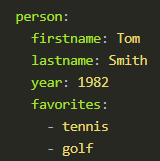
\includegraphics[scale=1]{../figures/5SC.png} }

\caption{Contoh Source Code} 
\label{Sc}
\end{figure}

Pada gambar \ref{Sc} dijelaskan tentang Contoh Source Code.

\subsection{Definisi Lain dari YAML}
YAML merupakan format serial data yang dapat dibaca oleh manusia yang mengambil beberapa bahas apemrograman seperti XML, C, Python, serta format email seperti yang recantum dalam RFC 2822. Pengusul YAML adalah Clark Evans pada tahun2001 silam. Clark merancang format ini bersama dengan Ingy döt Net dan Oren Ben-Kiki. YAML pula tersedia dalam beberapa Bahasa dan script pemrograman.
\subsection{YAML}
YAML mengintegrasikan dan membangun berdasarkan konsep yang dijelaskan oleh bahasa C, Java, Perl, Python, Ruby, RFC0822 (MAIL), RFC1866 (HTML),RFC2045 (MIME), RFC2396 (URI), XML, SAX, SOAP, dan JSON.
Sintaks YAML motivated oleh Internet Mail (RFC0822) dan tetap sebagian kompatibel dengan standar itu. selanjutnya, meminjam dari MIME (RFC2045), produksi tingkat atas YAML adalah aliran dokumen independen, ideal untuk pesan berbasissistem pemrosesan terdistribusi.
\subsection{Definisi YAML}
Pada saat awal-awal perkembangan, YAML diartikan dari banyak orang adalah sebuah singkatan yaitu "Yet Another Markup Language". Namun seiring berkembangnya zaman, untuk memberitahu tujuannya lebih jauh yang terfokus pada data dan bukan markah dokumen, akhirnya singkatan YAML diubah menjadi "YAML Ain't a Markup Language." YAML tersedia untuk beberapa Bahasa dan skrip pemrograman.
\subsection{YAML}
Dari pembahasan di atas, yang telah membahas tentang JSON atau JavaScript Object Notation dan YAML atau YAML Aint Markup Language. Berdasarkan pembahasan di atas dapat di temukan perbedaan antara keduanya. Berikut adalah beberapa perbedaan yang dapat kami kemukakan :
Berikut adalah tabel \ref{table:perbedaan} perbedaan JSON dan YAML.
\begin{table}[h]
\caption{Perbedaan JSON dan YAML}

\centering
\begin{tabular}{ccc}
\hline
&JSON&YAML\\
\hline
Kegunaan&Cocok untuk Format Serialisasi&Cocok untuk konfigurasi\\
\hline
Fitur&tidak memiliki komentar, aliasing&memiliki komentar, aliasing \\
&dan anchoring, dan  mergering& dan anchoring, dan  mergering\\
\hline
\end{tabular}
\label{table:perbedaan}
\end{table}

\end{document}
